\documentclass[11pt,aspectratio=169,handout]{beamer}

\usetheme{Singapore}
\usecolortheme{orchid}

\usepackage[utf8]{inputenc}
\usepackage[russian]{babel}
\usepackage{amsmath}
\usepackage{amsfonts}
\usepackage{amssymb}
\usepackage{graphicx}
\usepackage{bibentry}
\usepackage{wasysym}
\usepackage[most]{tcolorbox}
\usepackage[normalem]{ulem}

\usepackage{hyperref}

\definecolor{info}{RGB}{62, 180, 137}
\definecolor{warn}{RGB}{128, 0, 0}

\author{Николай Анохин}
\title{Нейросетевые рекомендеры 2: \\ ранкеры и контент}

\logo{
\includegraphics[width=.05\textwidth]{images/ok_logo.png}}

\AtBeginSection[]{
  \begin{frame}
  \vfill
  \centering
  \begin{beamercolorbox}[sep=8pt,center,shadow=true,rounded=true]{title}
    \usebeamerfont{title}\insertsectionhead\par
  \end{beamercolorbox}
  \vfill
  \end{frame}
}

\begin{document}

{
\setbeamertemplate{headline}{}

\begin{frame}
\titlepage
\end{frame}

%\begin{frame}
%\tableofcontents
%\end{frame}

}

\begin{frame}{Контекст}

\begin{center}
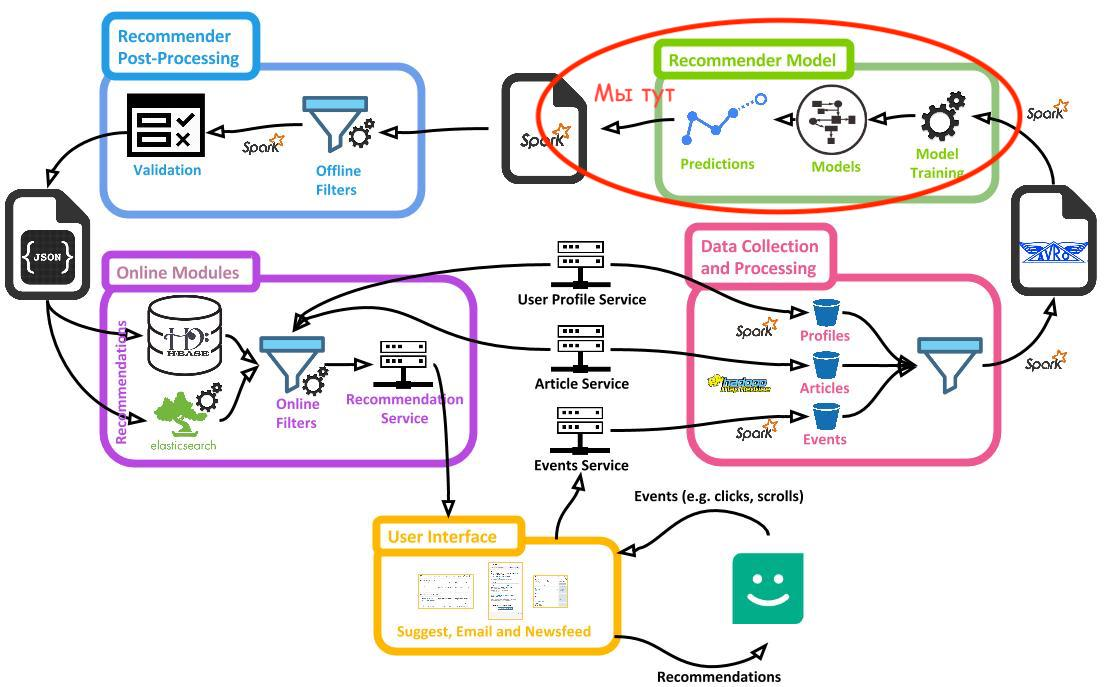
\includegraphics[scale=0.23]{images/mendeley.jpeg}
\end{center}

\end{frame}


\section{Истории успеха: ранжирование}

\begin{frame}{Постановка задачи ранжирования}

\begin{columns}

\begin{column}{0.45\textwidth} 
\begin{center}
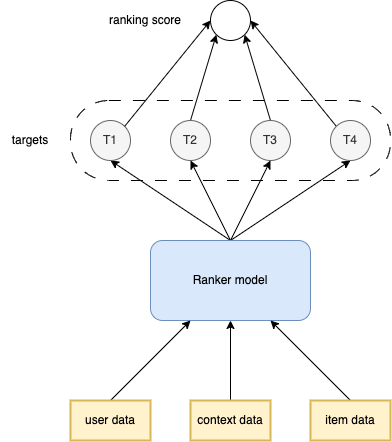
\includegraphics[scale=0.3]{images/ranker-framework.png}
\end{center}
\end{column}

\begin{column}{0.45\textwidth}
{\bf Задача} \\
Выбрать порядок кандидатов так, чтобы самые релевантные стояли в голове списка.
\end{column}

\end{columns}

\end{frame}

\begin{frame}{Истории успеха: ранжирование}

\begin{tcolorbox}[colback=info!5,colframe=info!80,title=Как оставить след в науке]
\begin{itemize}
\item Победить xgboost
\item Пофиксить смещения
\end{itemize}
\end{tcolorbox}

\end{frame}

\begin{frame}{Applying Deep Learning To Airbnb Search \cite{AIRBNB}}

\begin{columns}
\begin{column}{0.45\textwidth} 
\begin{center}
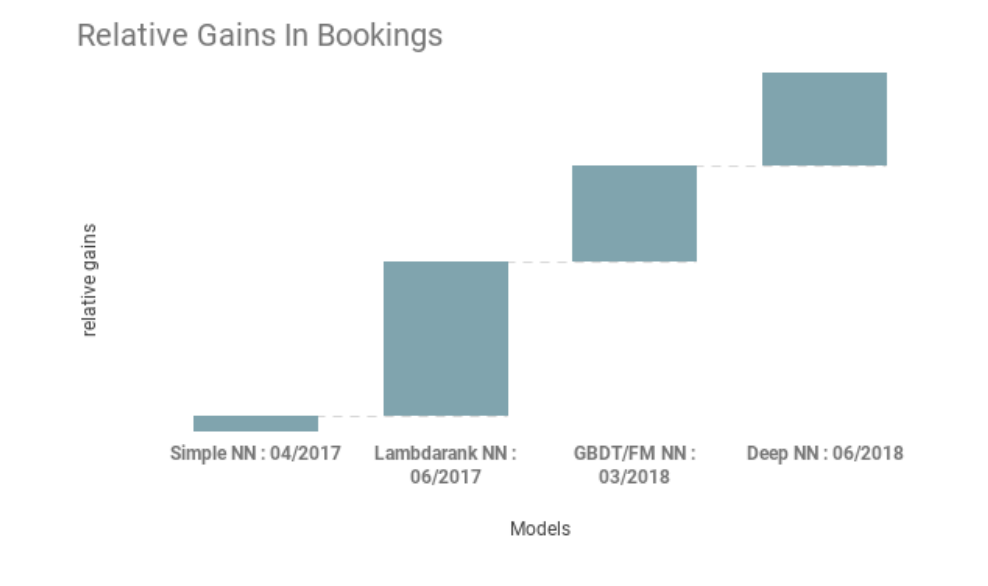
\includegraphics[scale=0.3]{images/airbnb-progression.png}
\end{center}
\end{column}
\begin{column}{0.45\textwidth}
\begin{center}
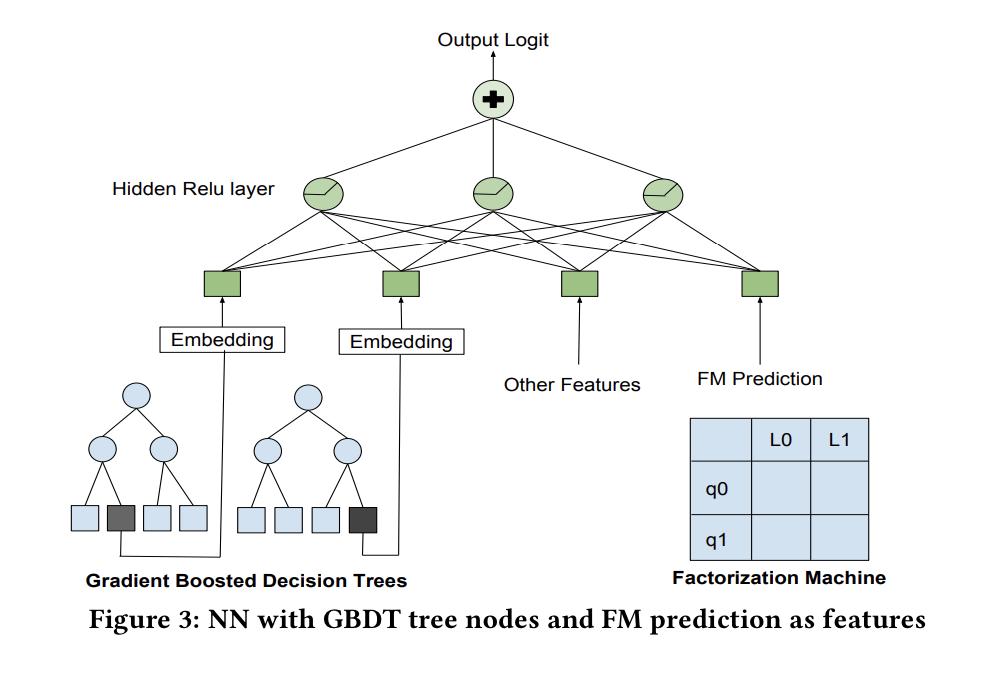
\includegraphics[scale=0.3]{images/airbnb-gbdt.png}
\end{center}
\end{column}
\end{columns}

\begin{tcolorbox}[colback=info!5,colframe=info!80,title=]
...we were able to deprecate all that complexity by simply scaling the training data 10x and moving to a DNN with 2 hidden layers...
\end{tcolorbox}

\vfill
\begin{small}
\begin{tabular}{l l}
Идея & Специфика применения NN ранкера на практике \\
Интересность & $\star\star\star\star$ \\
Полезность & $\star\star\star\star\star$
\end{tabular}
\end{small}

\end{frame}

\begin{frame}{Wide \& Deep Learning: Better Together with TensorFlow \cite{WD}}

\begin{center}
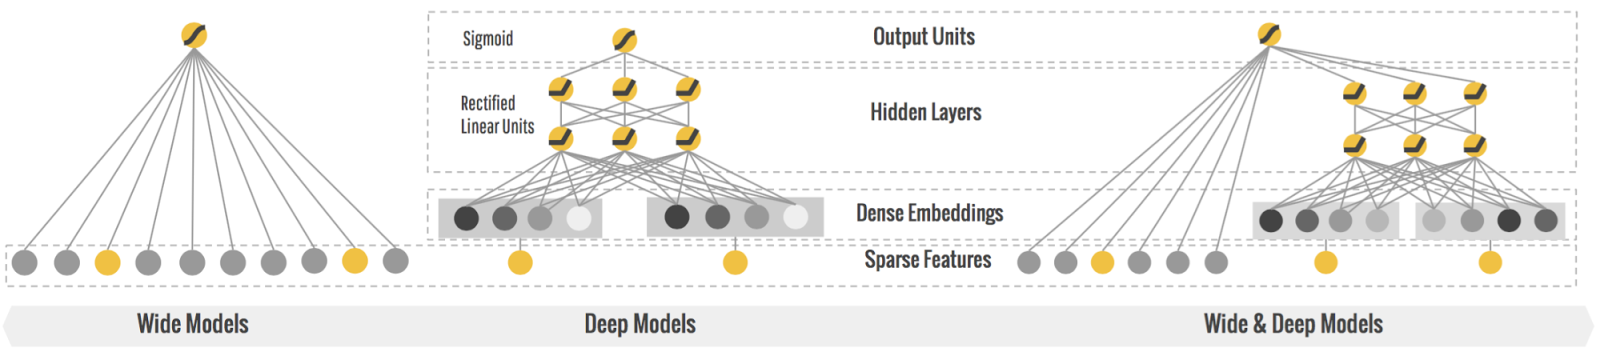
\includegraphics[scale=0.25]{images/widedeep.png}
\end{center}

\vfill
\begin{small}
\begin{tabular}{l l}
Идея & Скомбинировать ``ручные'' перемножения признаков с нелинейностью NN \\
Интересность & $\star\star$ \\
Полезность & $\star\star\star$
\end{tabular}
\end{small}

\end{frame}

\begin{frame}{DCN V2: Improved Deep \& Cross Network and Practical Lessons for Web-scale Learning to Rank Systems \cite{DCN}}

\begin{columns}
\begin{column}{0.45\textwidth} 
\begin{center}
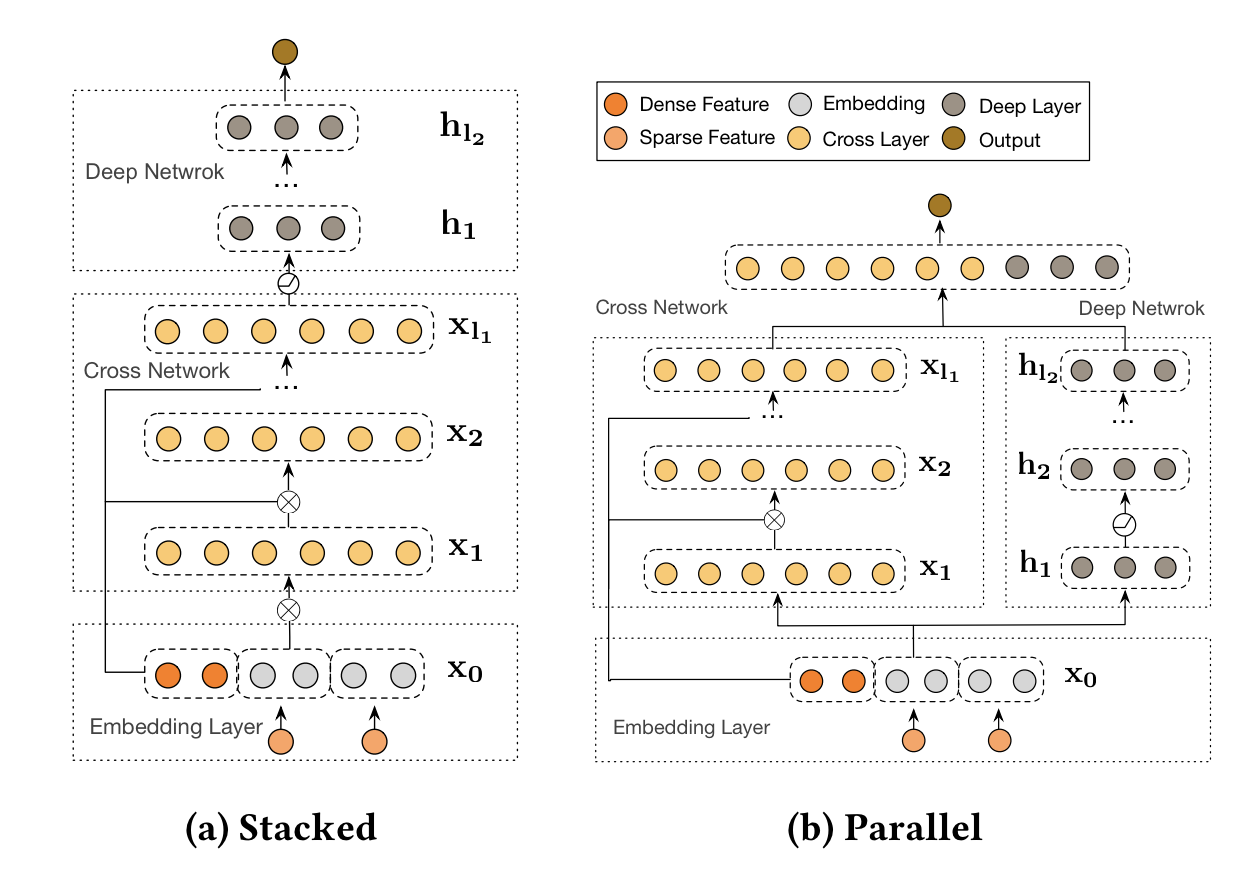
\includegraphics[scale=0.3]{images/dcn-arch.png}
\end{center}
\end{column}
\begin{column}{0.45\textwidth}
\begin{center}
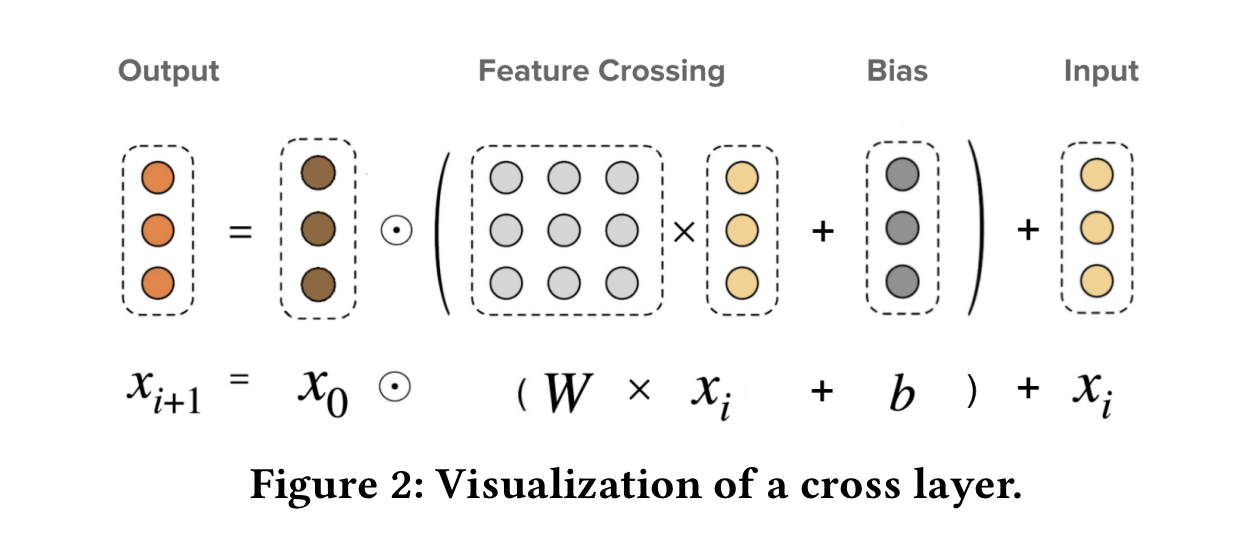
\includegraphics[scale=0.3]{images/dcn-block.png}
\end{center}
\end{column}
\end{columns}

\vfill
\begin{small}
\begin{tabular}{l l}
Идея & Интегрировать перемножения признаков в архитектуру NN \\
Интересность & $\star\star\star$ \\
Полезность & $\star\star\star\star$
\end{tabular}
\end{small}

\end{frame}

\begin{frame}{YouTube: ранжирование}

\begin{center}
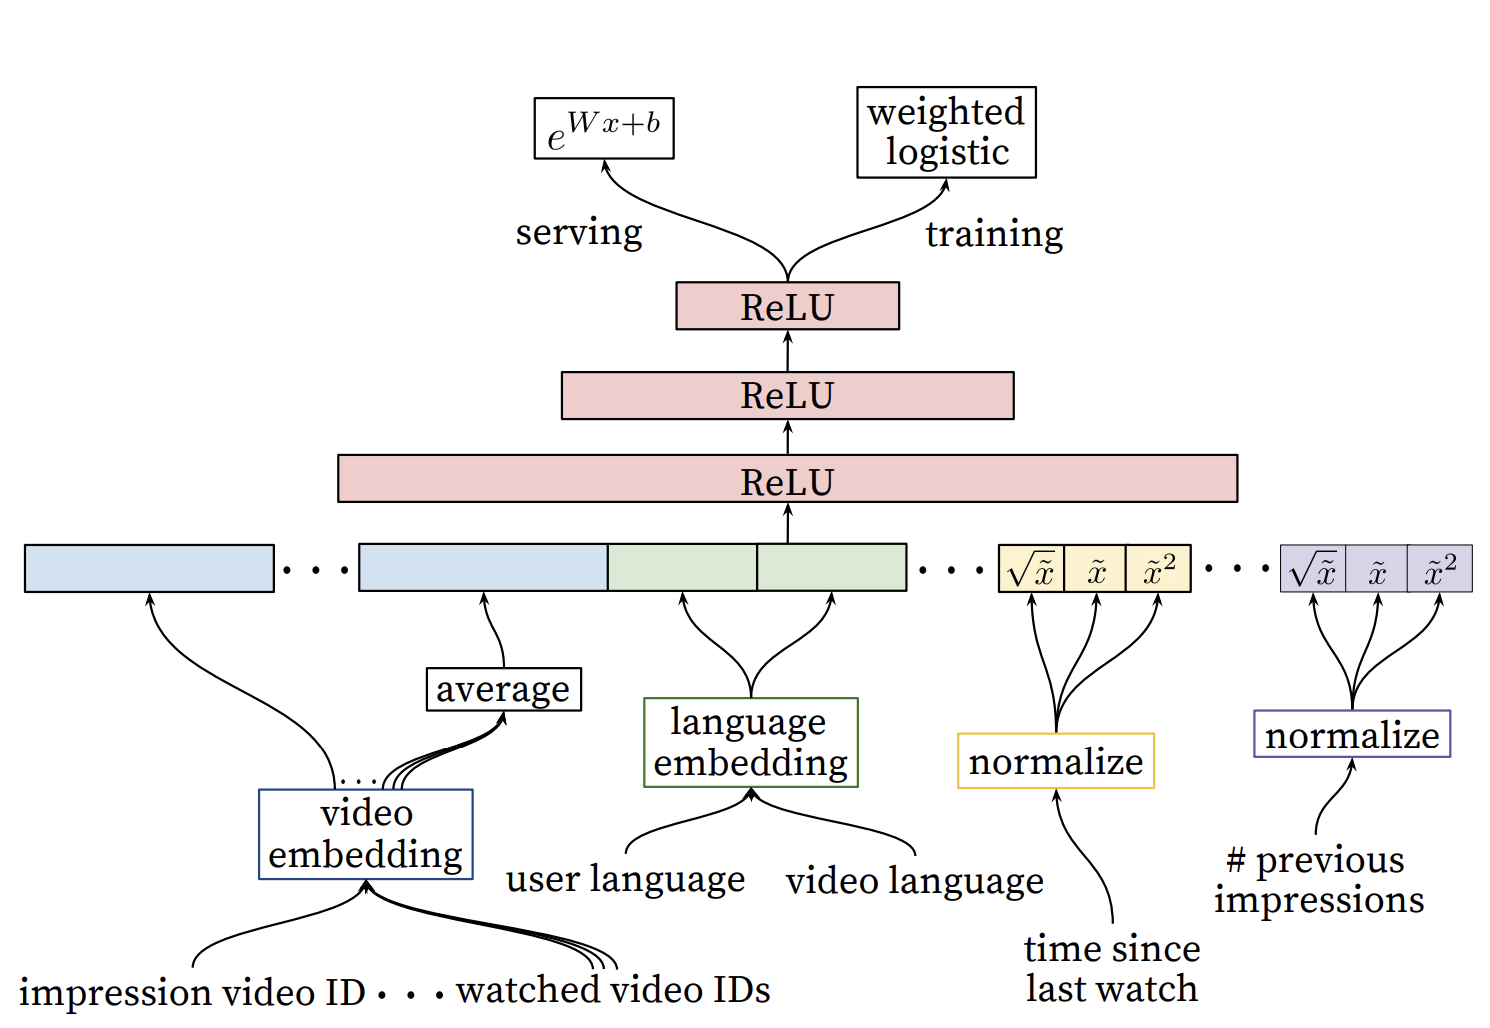
\includegraphics[scale=0.3]{images/youtube-rank.png}
\end{center}

\vfill
\begin{small}
\begin{tabular}{l l}
Идея & Использовать последовательность айтемов как признак \\
Интересность & $\star\star\star\star\star$ \\
Полезность & $\star\star\star\star\star$
\end{tabular}
\end{small}

\end{frame}

\begin{frame}{Механизм attention \cite{NMT}}

\begin{columns}
\begin{column}{0.45\textwidth} 
\begin{center}
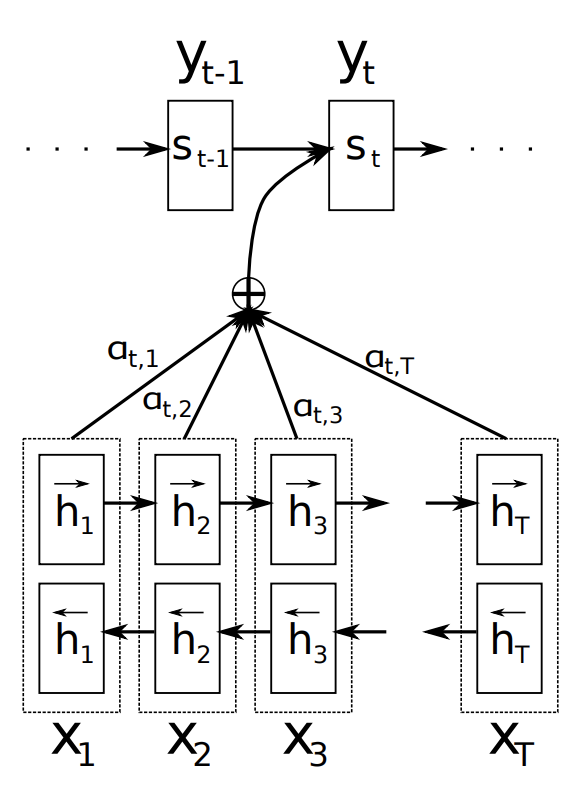
\includegraphics[scale=0.3]{images/nmt-arch.png}
\end{center}
\end{column}
\begin{column}{0.45\textwidth}
\begin{center}
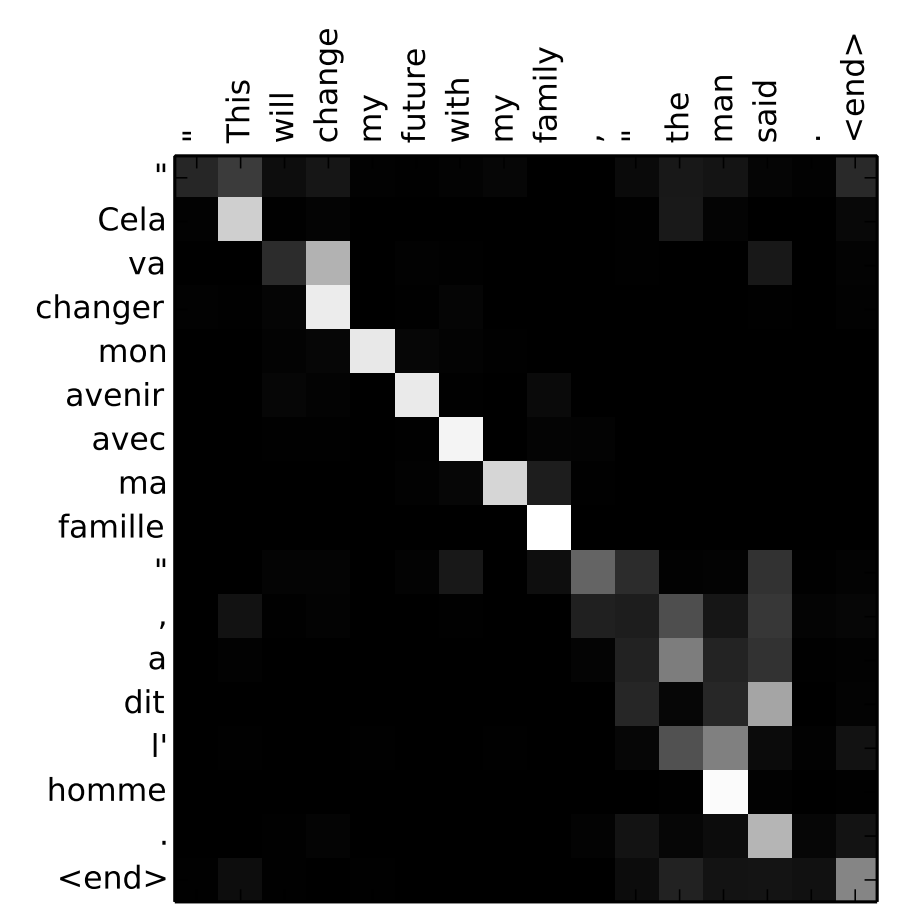
\includegraphics[scale=0.3]{images/nmt-example.png}
\end{center}
\end{column}
\end{columns}

\vfill
\[
\alpha_{ij} = \frac{\exp e_{ij}}{\sum_k \exp e_{ik}}, \quad e_{ij} = ffn(s_{i-1}, h_j)
\]

\end{frame}

\begin{frame}{Deep Interest Network for Click-Through Rate Prediction \cite{DIN}}

\begin{center}
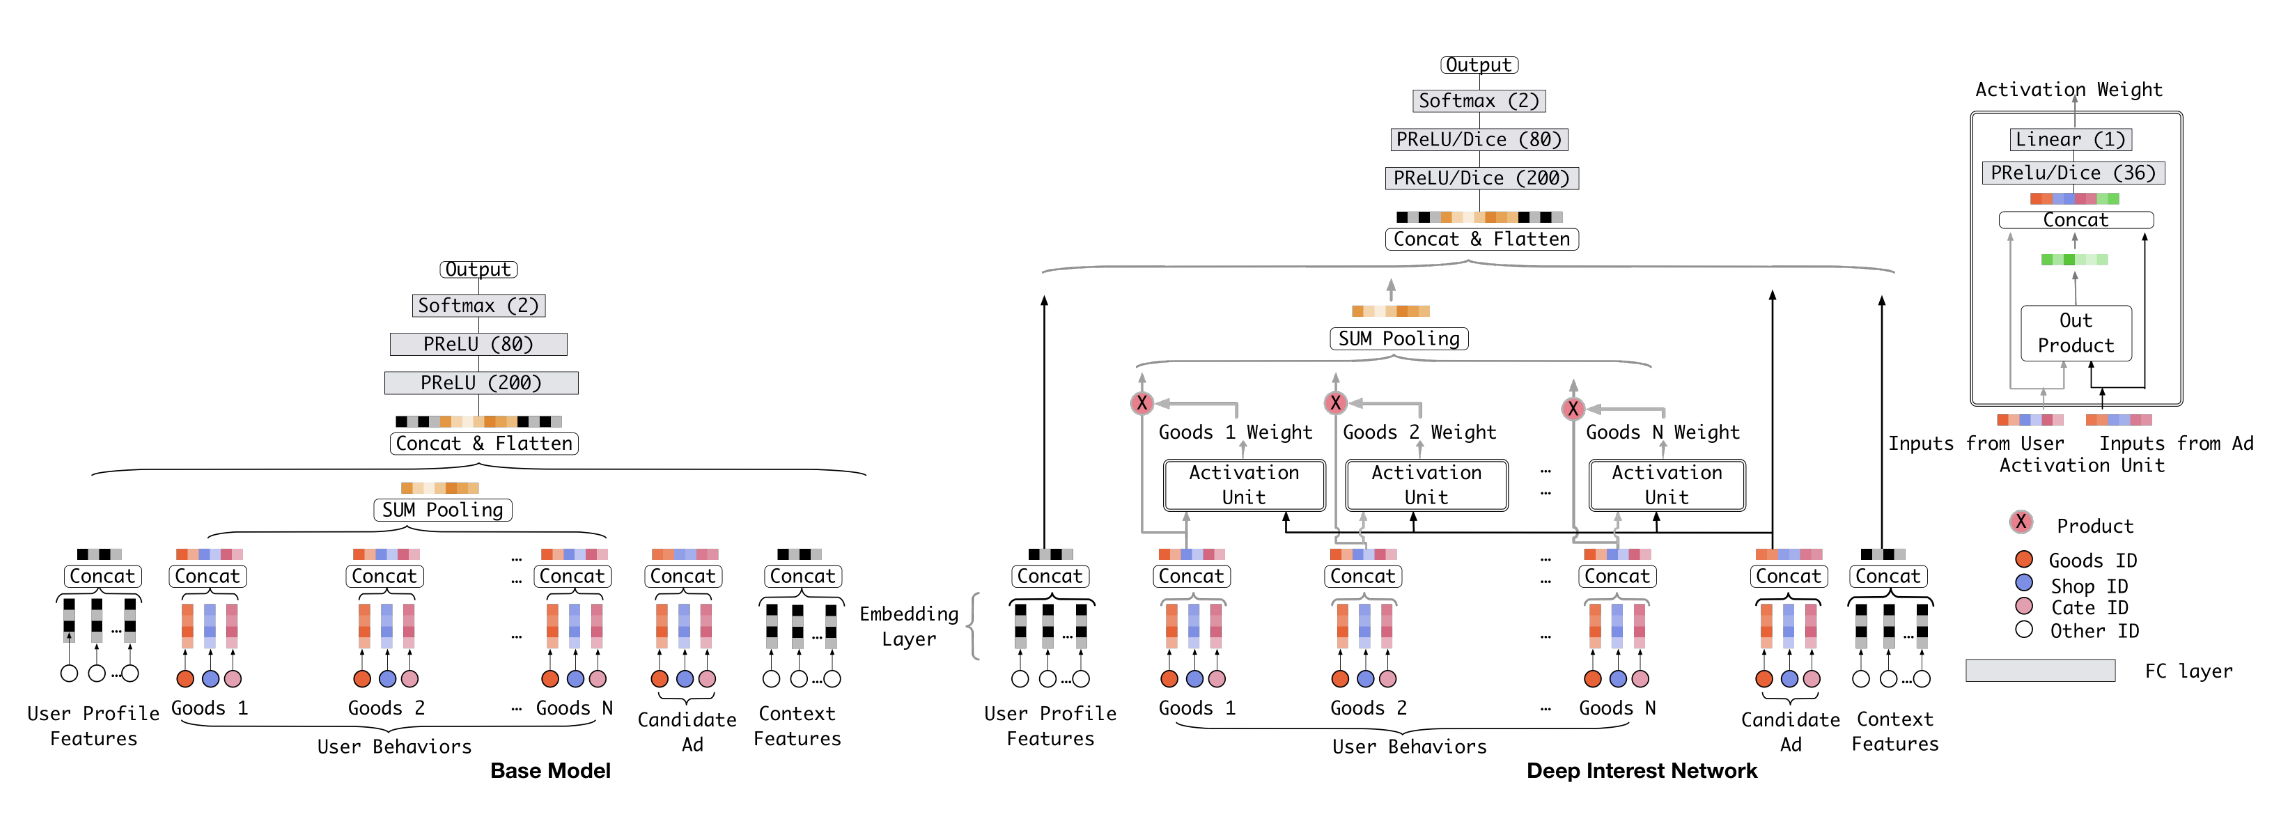
\includegraphics[scale=0.3]{images/din.png}
\end{center}

\vfill
\begin{small}
\begin{tabular}{l l}
Идея & Attention (почти) для агрегации последовательности айтемов \\
Интересность & $\star\star\star\star$ \\
Полезность & $\star\star\star\star$
\end{tabular}
\end{small}

\end{frame}

\begin{frame}{MaskNet: Introducing Feature-Wise Multiplication to CTR Ranking Models by Instance-Guided Mask \cite{MASKNET}}

\begin{columns}
\begin{column}{0.45\textwidth} 
\begin{center}
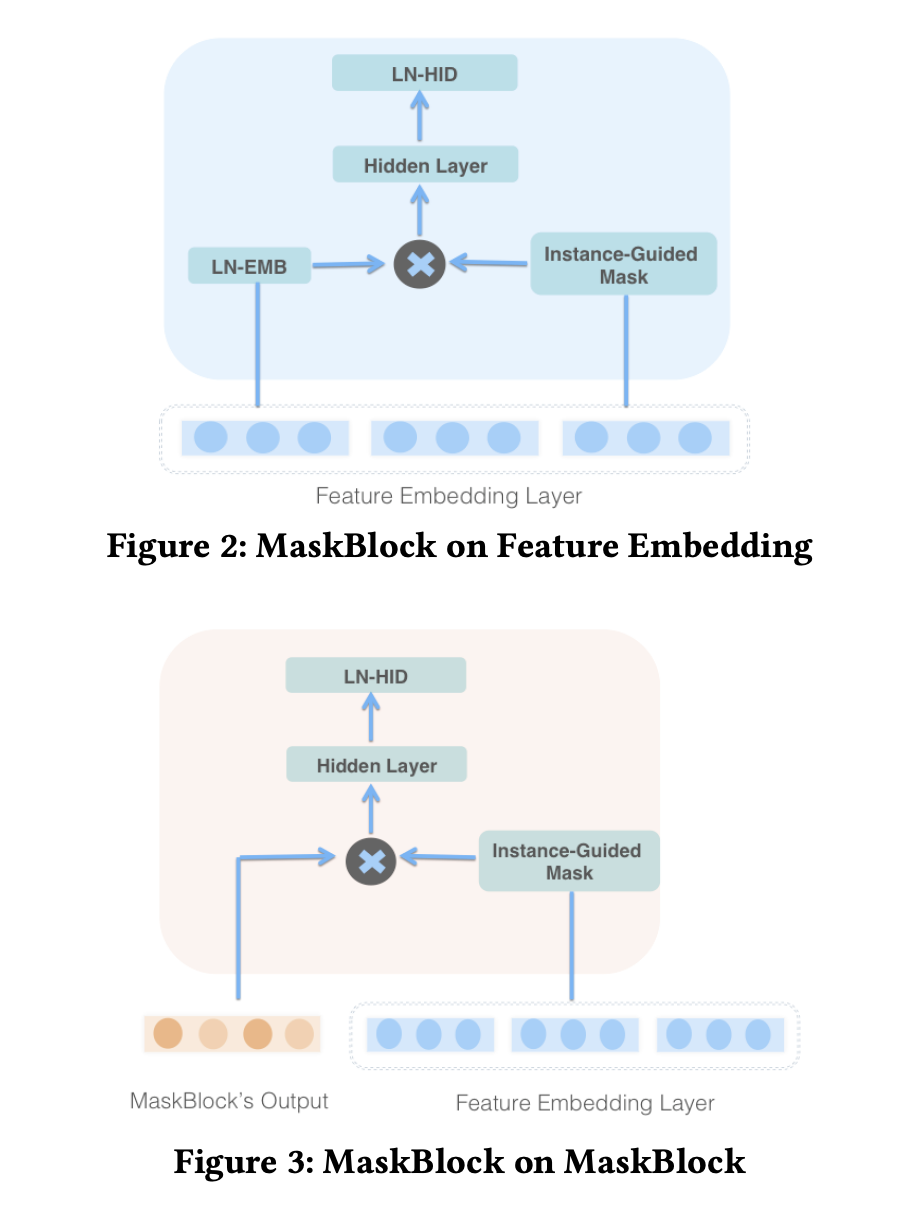
\includegraphics[scale=0.25]{images/mask-block.png}
\end{center}
\end{column}
\begin{column}{0.45\textwidth}
\begin{center}
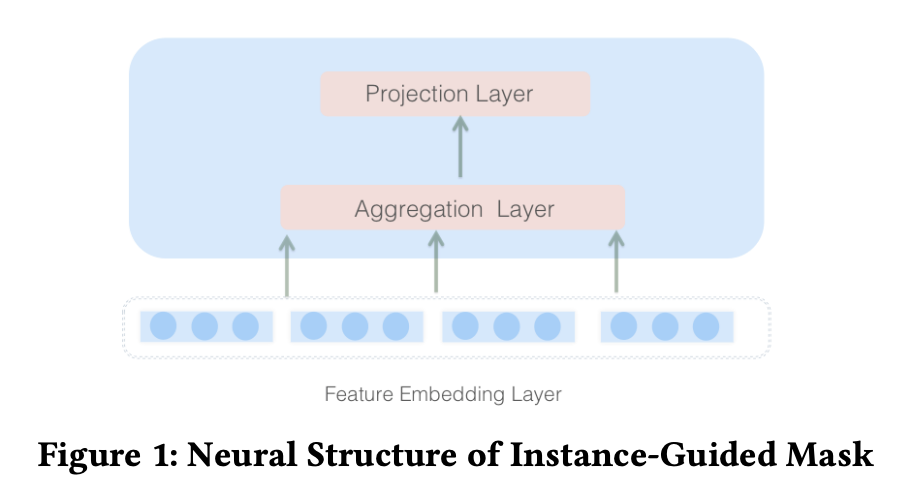
\includegraphics[scale=0.3]{images/mask-mask.png}
\end{center}
\end{column}
\end{columns}

\end{frame}

\begin{frame}{MaskNet: Introducing Feature-Wise Multiplication to CTR Ranking Models by Instance-Guided Mask \cite{MASKNET}}

\begin{center}
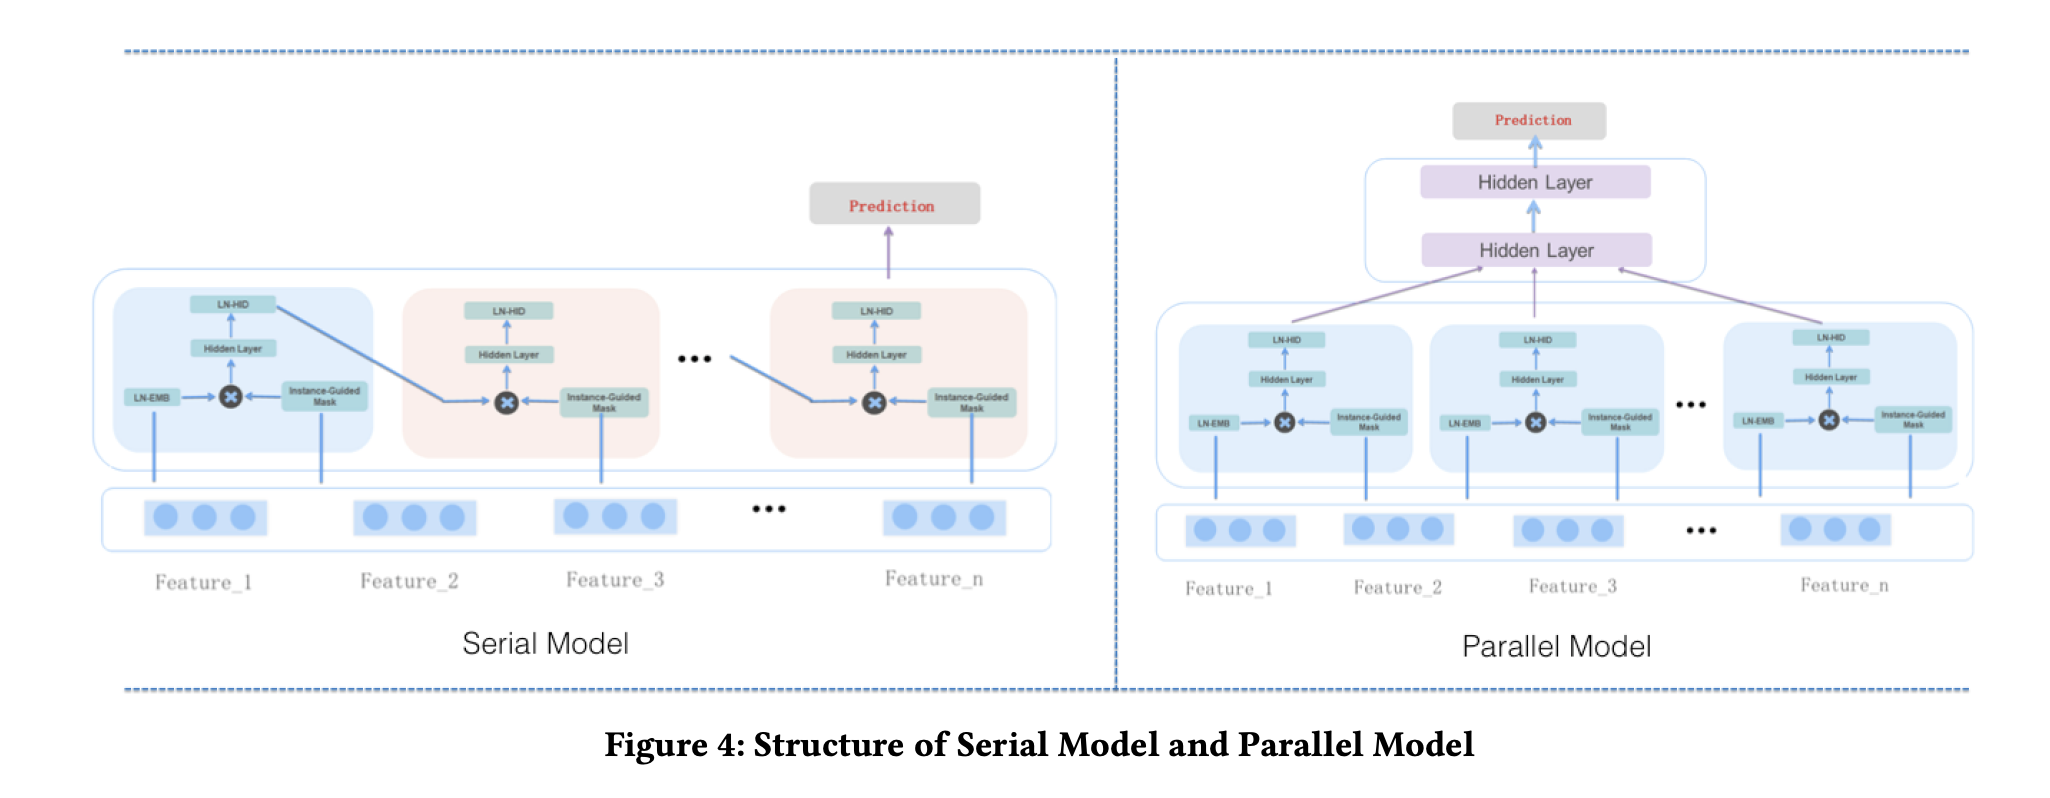
\includegraphics[scale=0.3]{images/mask-arch.png}
\end{center}

\vfill
\begin{small}
\begin{tabular}{l l}
Идея & Обучаемая маска выбирает ``полезные'' части выходов слоя \\
Интересность & $\star\star\star\star$ \\
Полезность & $\star\star\star\star$
\end{tabular}
\end{small}

\end{frame}

\begin{frame}{Recommending What Video to Watch Next: A Multitask Ranking System \cite{RANKING}}

\begin{center}
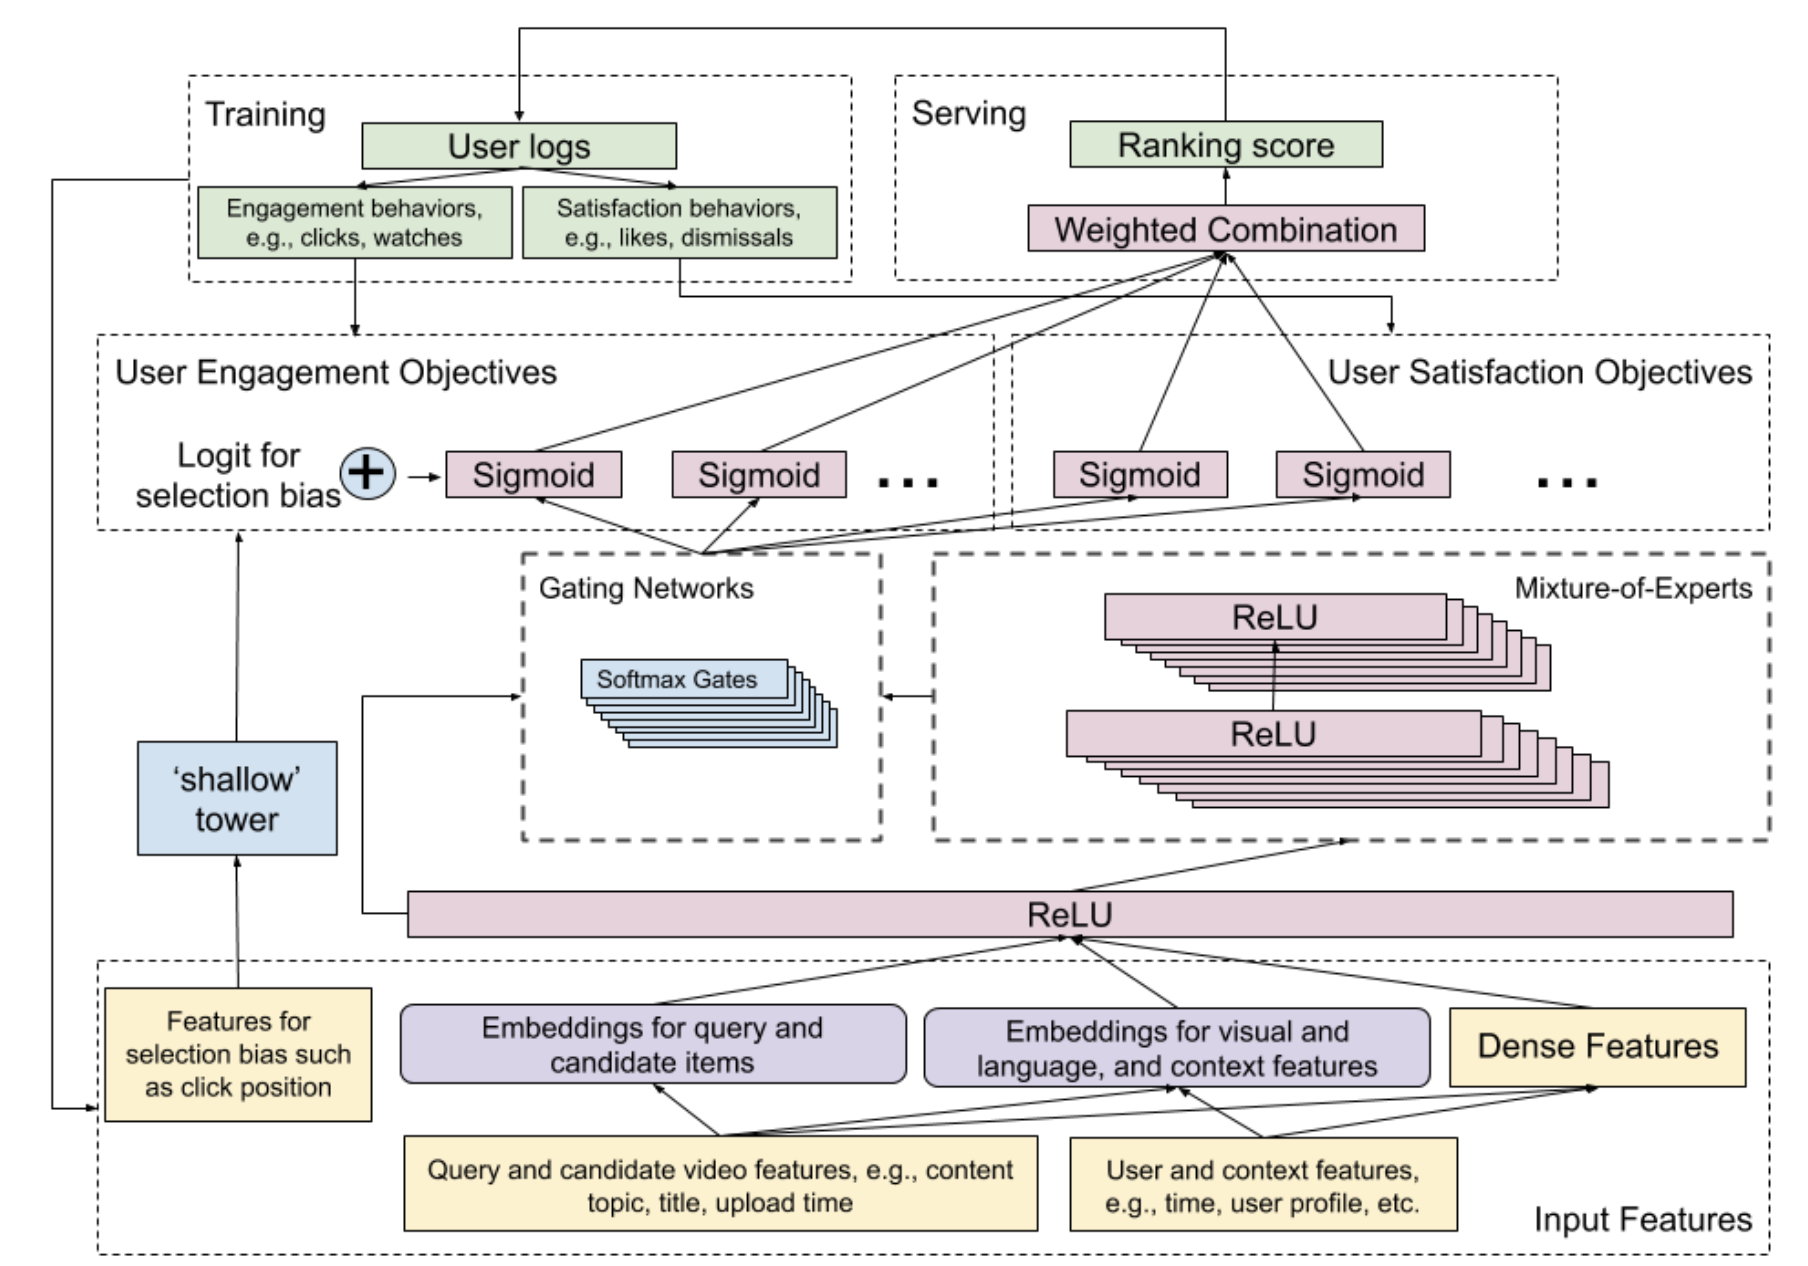
\includegraphics[scale=0.2]{images/multitask.png}
\end{center}

\vfill
\begin{small}
\begin{tabular}{l l}
Идея & Attention выбирает экспертов под разные таргеты \\
Интересность & $\star\star\star\star\star$ \\
Полезность & $\star\star\star\star$
\end{tabular}
\end{small}

\end{frame}

\section{Истории успеха: контент}

\begin{frame}{Истории успеха: контент}

\begin{tcolorbox}[colback=info!5,colframe=info!80,title=Как оставить след в науке]
\begin{itemize}
\item Решить проблему холодного старта, хитро обучив эмбединги
\end{itemize}
\end{tcolorbox}

\end{frame}

\begin{frame}{Learning Transferable Visual Models From Natural Language Supervision \cite{CLIP}}

\begin{center}
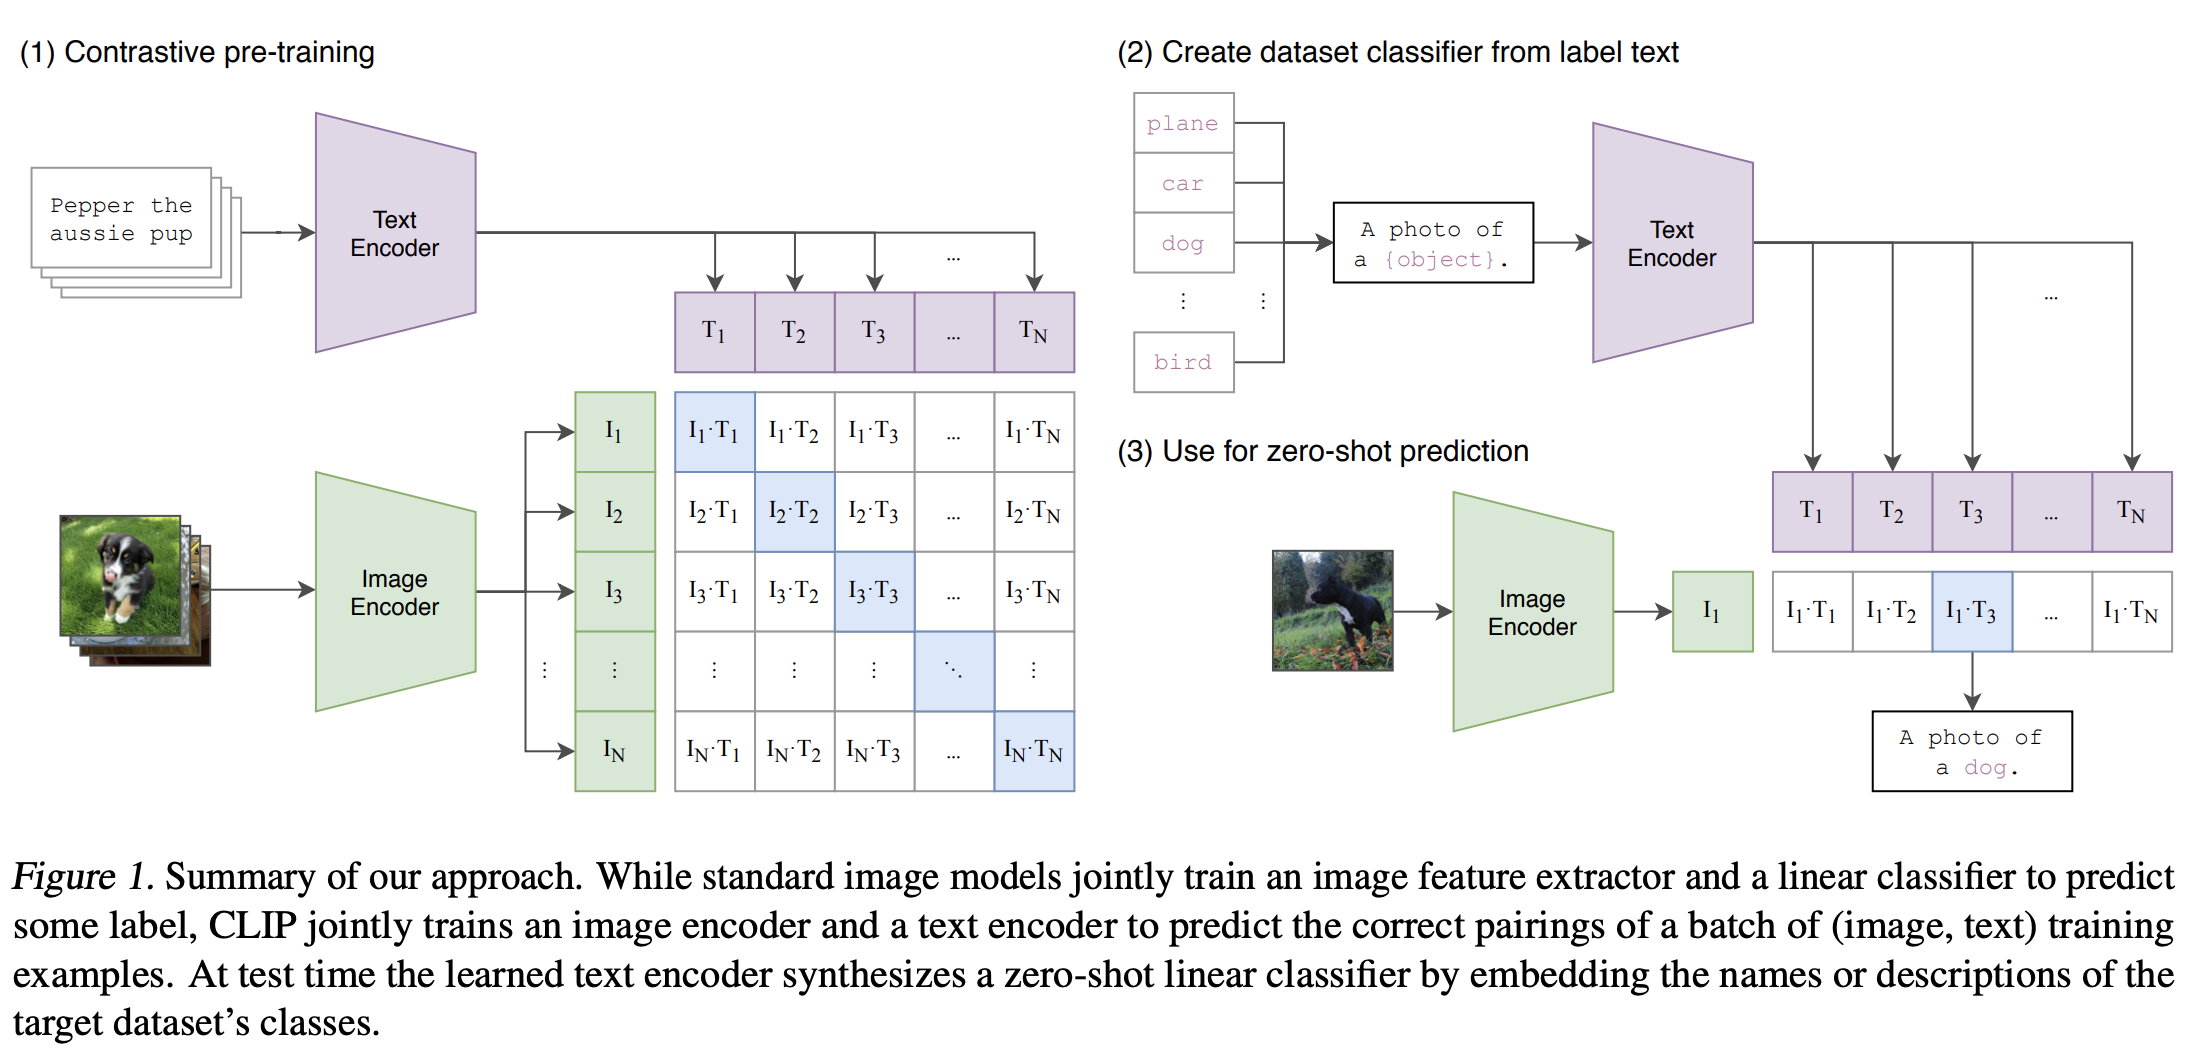
\includegraphics[scale=0.25]{images/clip.png}
\end{center}

\vfill
\begin{small}
\begin{tabular}{l l}
Идея & Мульти-модальные эмбеддинги решают вопросы \\
Интересность & $\star\star\star$ \\
Полезность & $\star\star\star$
\end{tabular}
\end{small}

\end{frame}

\begin{frame}{CB2CF: A Neural Multiview Content-to-Collaborative Filtering Model for Completely Cold Item Recommendations \cite{CB2CF}}

\begin{center}
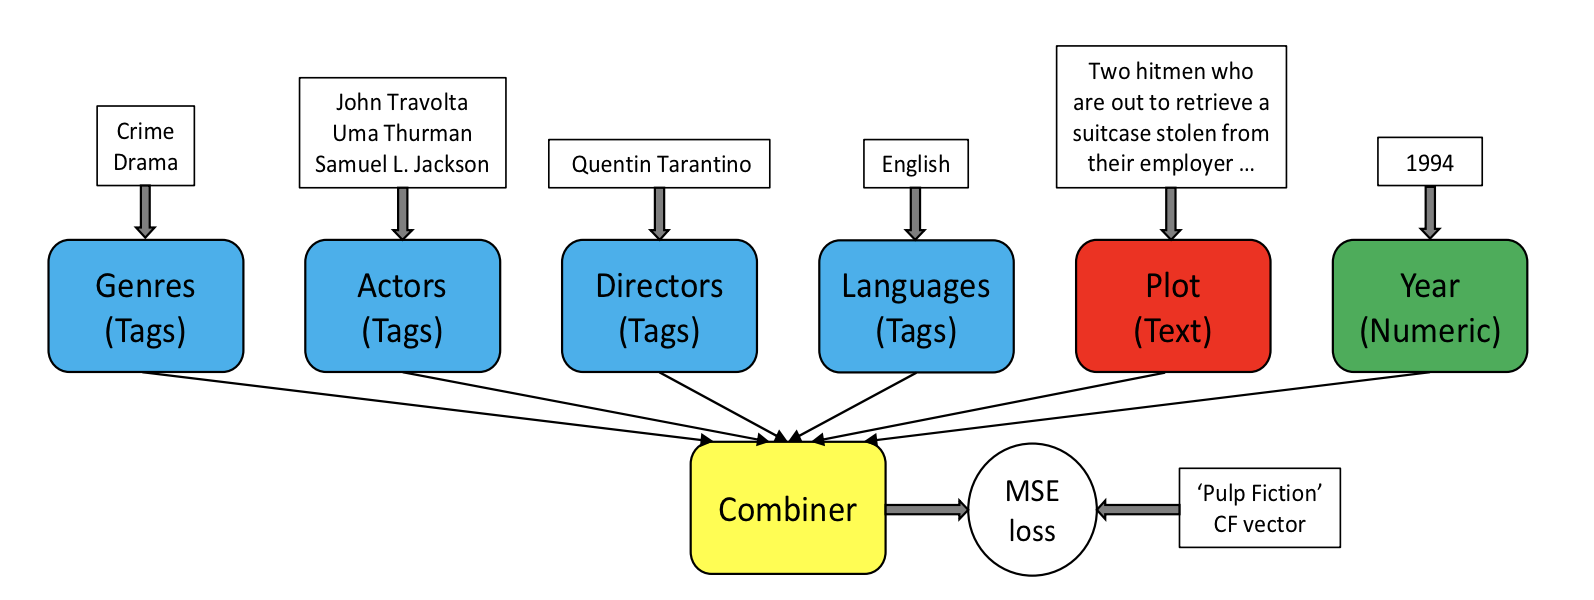
\includegraphics[scale=0.4]{images/cf2cf.png}
\end{center}

\vfill
\begin{small}
\begin{tabular}{l l}
Идея & Использум результат коллаборативной модели для обучения контентной \\
Интересность & $\star\star\star\star$ \\
Полезность & $\star\star\star\star\star$
\end{tabular}
\end{small}

\end{frame}

\section{Что работает на практике}

\begin{frame}{Архитектуры \cite{METH}}

\begin{itemize}
\item Мульти-таргет решает.
\item Авто пересечение признаков (DCN, MaskNet).
\item MoE не дает профита при том же количестве параметров, как у базовых архитектур.
\item DIN дает эффект для длинных последовательностей.
\end{itemize}

\end{frame}

\begin{frame}{Improving Deep Learning For Airbnb Search \cite{AIRBNB2}}

\begin{tcolorbox}[colback=warn!5,colframe=warn!80,title=]
If deeper nets were not the right architecture for us, we hypothesized, more specialized architectures might be. 
So we tried architectures [...] like {\bf deep and wide} [...] followed by variants of {\bf attention based networks}. 
[...] The short summary of those efforts is that they {\bf failed to move the needle}.
\end{tcolorbox}

\vfill
\begin{small}
\begin{tabular}{l l}
Идея & Архитектура должна следовать из проблемы пользователя \\
Интересность & $\star\star\star\star\star$ \\
Полезность & $\star\star\star\star\star$
\end{tabular}
\end{small}

\end{frame}

\section{Проблемы нейрорекомендеров}

\begin{frame}{Проблема воспроизводимости \cite{PROGRESS}}

\begin{tcolorbox}[colback=warn!5,colframe=warn!80,title=]
Многие результаты из статей невозможно воспроизвести
\end{tcolorbox}

\begin{tcolorbox}[colback=warn!5,colframe=warn!80,title=]
Некоторые новые алгоритмы работают хуже, чем затюненные бейзлайны
\end{tcolorbox}

\begin{columns}
\begin{column}{0.45\textwidth} 
\begin{tcolorbox}[colback=gray!5,colframe=gray!80,title=]
The CMN method was presented at SIGIR 18 and combines memory networks and neural attention mechanisms with latent factor and neighborhood models
\end{tcolorbox}
\end{column}
\begin{column}{0.45\textwidth}
\begin{center}
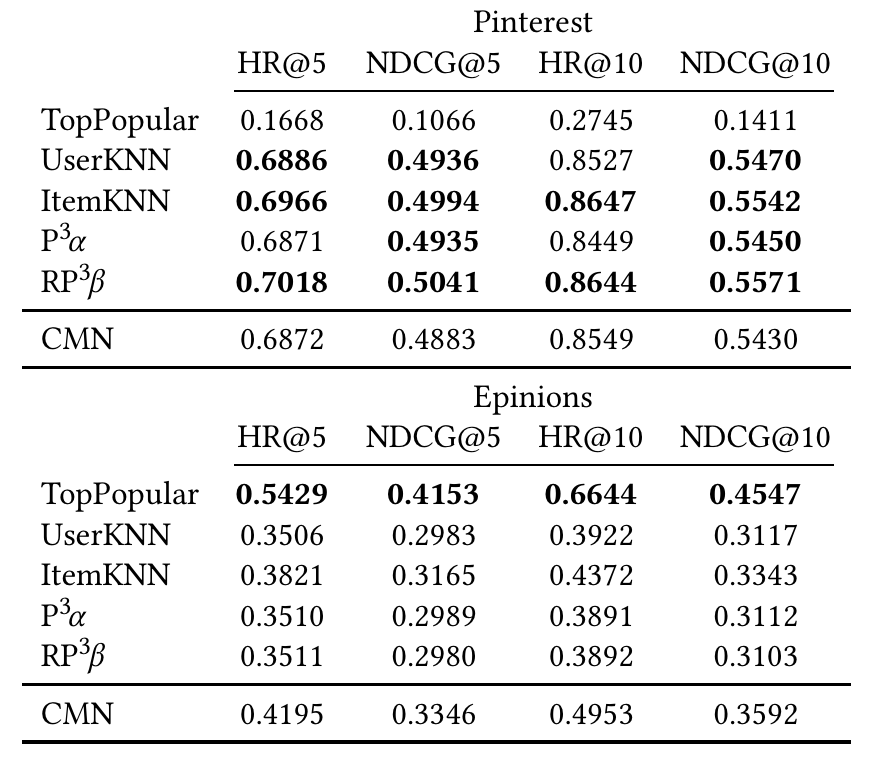
\includegraphics[scale=0.25]{images/progress.png}
\end{center}
\end{column}
\end{columns}

\end{frame}

\begin{frame}{Проблема сравнений \cite{DALMANN}}

\begin{tcolorbox}[colback=warn!5,colframe=warn!80,title=]
Результат сравнения может поменяться на обратный в зависимости от того, по какой метрике сравнивають
\end{tcolorbox}

\begin{center}
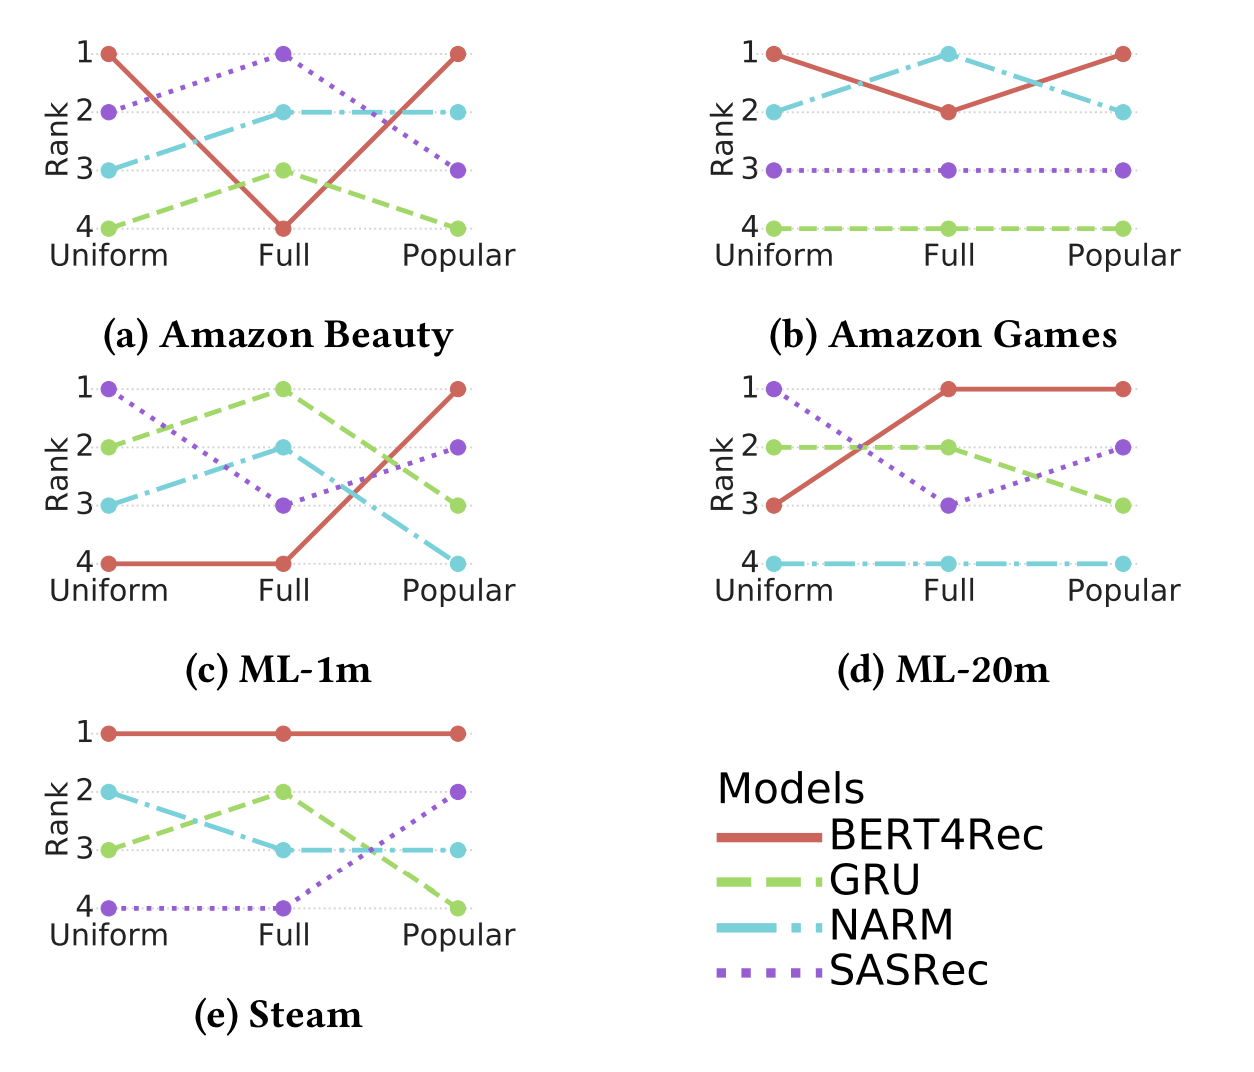
\includegraphics[scale=0.25]{images/compare.png}
\end{center}

\end{frame}

\section{Итоги}

\begin{frame}{Итоги}

\begin{tcolorbox}[colback=info!5,colframe=info!80,title=]
Нейросетевые модели могут заменить любой компонент рекомендательной системы: отборщик кандидатов, ранкер, item2item.
\end{tcolorbox}

\begin{tcolorbox}[colback=warn!5,colframe=warn!80,title=]
Нейросетевой подход не гарантирует выигрыша -- к выбору модели нужно подходить прагматично.
\end{tcolorbox}

\end{frame}

\begin{frame}{Феерически завершающий лекцию слайд}

\begin{columns}
\begin{column}{0.45\textwidth}
   \begin{center}
                
\includegraphics[scale=0.35]{images/bye.png}
   \end{center}
\end{column}
\begin{column}{0.45\textwidth}
   \begin{center}
                \url{https://t.me/mlvok}

                
\includegraphics[scale=0.5]{images/tgqr.png}
   \end{center}
\end{column}
\end{columns}

\end{frame}

\begin{frame}[allowframebreaks]{Литература}

\bibliographystyle{amsalpha}
\bibliography{references.bib}

\end{frame}

\end{document}
